% !TEX root = ../thesis-example.tex
%
%************************************************
% Evaluation
%************************************************
\chapter{Evaluation und Auswertung}
\label{sec:Evaluation}

\section{Einführung}
\label{sec:Evaluation:Einfuehrung}

In vorherigen Kapitel haben wir unseren Lösungsansatz in der Springermedizin-Suche implementiert. Wir wissen nun wie und warum wir den Reranking-Algorithmus umgesetzt haben. Was wir bisher nicht wissen ist, \textit{wie gut} er funktioniert. Mithilfe einer Evaluation wollen wir darum nun messen, wie gut die Suchergebnis-Qualität der aktuellen Springermedizin-Suche im Vergleich zur im Zuge dieser Arbeit entwickelten Lösung mit dem Reranking-Algorithmus ist. 

\subsubsection{Ziel der Evaluation}
\label{sec:Evaluation:Einfuehrung:Ziel}

Die Evaluation soll Informationen darüber liefern, wie viel Verbesserung der neue Lösungsansatz bringt. Aus den Ergebnissen wollen wir erkennen, was an dem Lösungsansatz geändert werden muss, damit die Suche wirklich gute Ergebnisse aus Sicht der User liefert und unter welchen Voraussetzungen, sie im Springermedizin-Umfeld eingesetzt werden kann.

\subsubsection{Methodik}
\label{sec:Evaluation:Einfuehrung:Methodik}
Wir werden durch fachliche Experten (Redakteure von Springermedizin) die Suchergebnisse von oft gesuchten Suchanfragen bewerten lassen. Dazu werden wir eine Testumgebung mit einem Evaluations-System und den beiden oben angesprochenen Suchvarianten aufbauen. Die Redakteure sollen bei der Evaluation, zu jeder Suchanfrage die ersten zehn Suchergebnisse analysieren und anhand der Suchsnippets, die Relevanz bewerten. Diese Analyse sollen sie jeweils einmal auf der aktuellen Springermedizin-Suche und einmal auf der Springermedizin-Suche mit dem Reranking-Algorithmus durchführen. Am Ende werden wir die Ergebnisse auswerten und einen Vergleich der beiden Suchvarianten machen. 

\section{Aufbau der Analyse}
\label{sec:Evaluation:Aufbau}

Mithilfe der Relevanz-Bewertungen wollen wir das Qualitätsmaß der Suchvarianten bestimmen. Dazu müssen wir zuerst die \glqq zuverlässigen\grqq{} Bewertungen mittels \textit{Kappa-Koeffizienten} filtern und dann mithilfe der \textit{nDCG-Metrik} auswerten. Der Prozess dazu sieht wie folgt aus:

\begin{figure}[H]
\centering
\vspace{-.5em}
\caption[Prozess der Datenaufbereitung und Metrik der Auswertung]{Prozess der Datenaufbereitung und Metrik der Auswertung}
\vspace{.5em}
\label{fig:SucheSpringerNature}
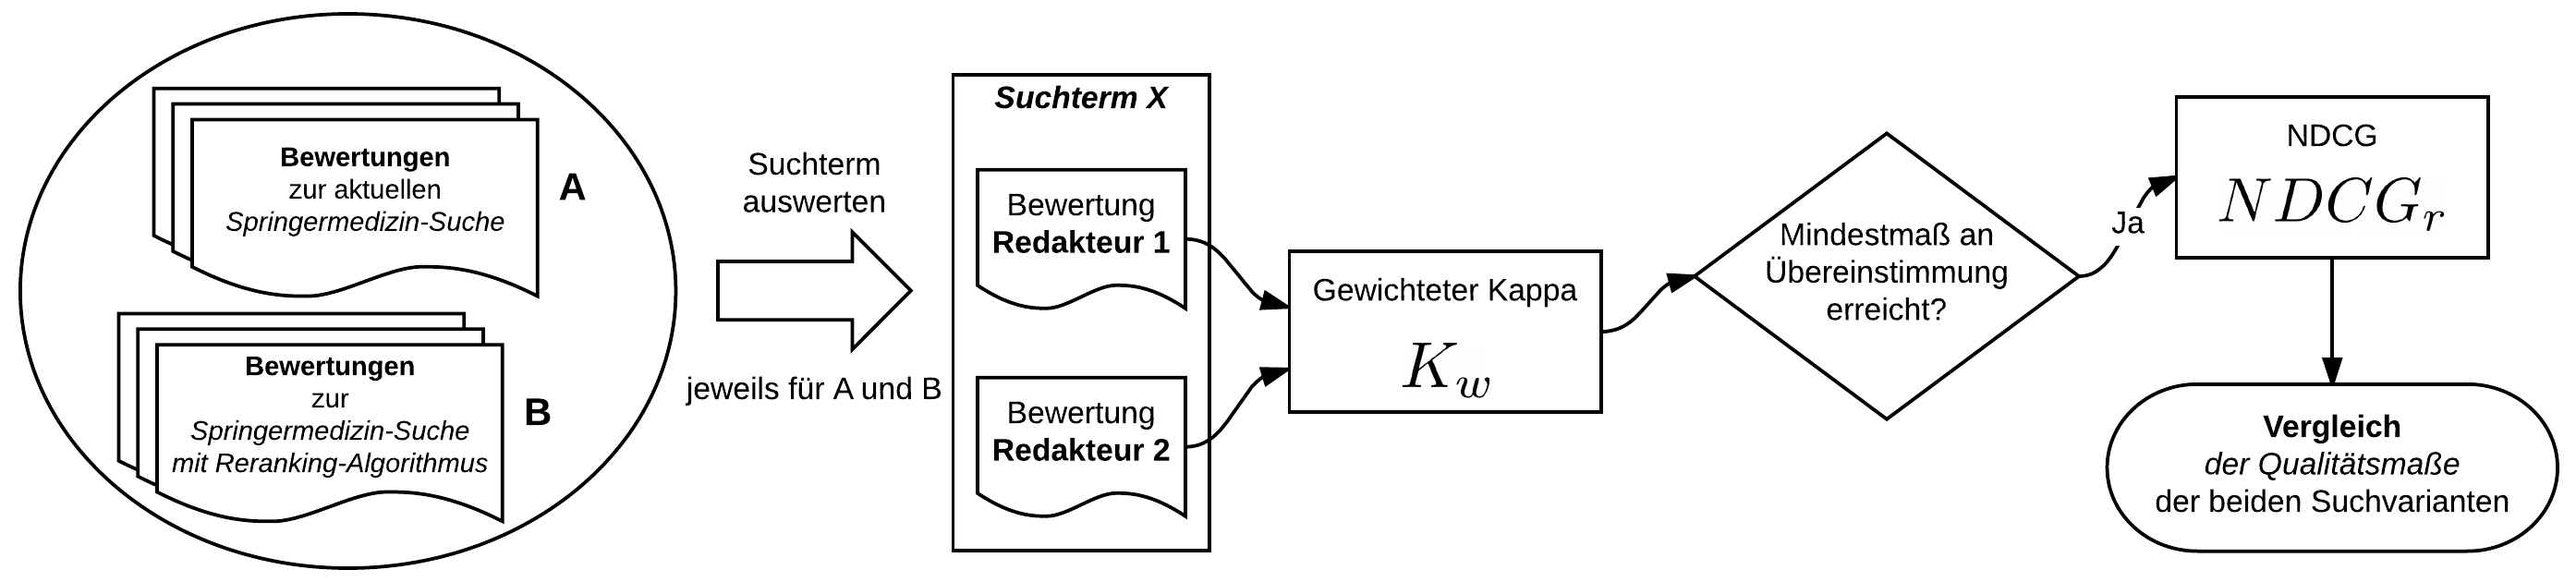
\includegraphics[width=\linewidth]{gfx/EvaluationDatenaufbereitung}
\vspace{-2em}
\end{figure}

\pagebreak

In diesem Kapitel werden Formeln eingeführt. Folgend eine Legende der wichtigsten Symbole:

\begin{table}[H]
\centering
\vspace{-.5em}
\caption[Legende der wichtigsten Formel-Symbolen für die Evaluation]{Legende der wichtigsten Formel-Symbolen für die Evaluation}
\label{tab:LegendeSymboleFormelnEvaluation}
\vspace{-.5em}
\footnotesize
\renewcommand*{\arraystretch}{1.2}
\resizebox{\textwidth}{!}{%
\begin{tabular}{llll}
\hline
\multicolumn{2}{l}{\textit{\textbf{Kappa}}}                            		& \multicolumn{2}{l}{\textit{\textbf{nDCG}}}                  \\ \hline
\textbf{Bedeutung} & \textbf{Symbol}                                   			& \textbf{Bedeutung} & \textbf{Symbol}                        \\ \hline
$K$				& Cohens-Kappa-Koeffizient     												& $r$                	& die Anzahl der zu prüfenden Positionen \\
$p_0$			& Anteil tatsächlich beobachteter Übereinstimmungen 			& $i$                	& die zu prüfende Position               \\               				
$p_e$			& Anteil zufälliger Übereinstimmungen               					& $rel_i$				& Relevanz-Wert der Position $i$             \\
$w$				& Gewichtung anhand der Abweichung zur Hauptdiagonale     & $REL$				& die Menge der Relevanz-Werte der Dokumente in $r$ in idealer Reihenfolge\\
$K_w$		& Gewichteter Cohens-Kappa-Koeffizient									& $DCG_r$     			& Discounted Cumulative Gain             \\ 
$R_i$		& Zeilensumme der Zeile $i$ in Übereinstimmungsmatrix					& $IDCG_r$    		& Ideal Discounted Cumulative Gain       \\
$C_i$		& Spaltensumme der Spalte $i$ in Übereinstimmungsmatrix				& $nDCG_r$  		& Normalized Discounted Cumulative Gain  \\\hline
\end{tabular}
}
\vspace{-2.5em}
\end{table}

\subsection{Hypothesen}
\label{sec:Evaluation:Aufbau:Hypothese}

\paragraph{Springermedizin-Content bietet keine optimale Grundlage für Relevanz-Bewertungen}
Aufgrund der Analysen der Click-Through-Daten und des Springermedizin-Contents in Kapitel \ref{sec:Grundlagen:Grundbegriffe}, wissen wir, dass wir keine optimale Grundlage für unseren Reranking-Algorithmus haben. Das liegt vor allem an den nicht beeinflussbaren Faktoren, wie die Ausspielung von Teasern mit geringer Aussagekraft und könnte sich vor allem in den Relevanz-Bewertungen der Suchergebnisse widerspiegeln. Da dieses Problem aber denselben Einfluss auf die aktuelle, sowie die neu implementierte Suche hat, sollte das Qualitätsmaß der nDCG-Auswertung davon nicht stark beeinflusst werden. 

\paragraph{Falsche Aussagen in den Click-Through-Daten verringern Qualitätsmaß des Reranking-Algorithmus}
Bei der Messung des Qualitätsmaßes mittels nDCG wird der Einfluss der Click-Through-Daten interessanter sein. Grundsätzlich müsste davon ausgegangen werden, dass viele Click-Through-Daten das Ergebnis positiv beeinflussen. Es sei denn, die verwendeten Click-Through-Daten beinhalten falsche Aussagen, da sie durch viele Klicks auf wenig relevante Suchergebnisse entstanden sind und wir die User-Aktivitäten nach einem Klick nicht messen können. Wir gehen darum davon aus, dass diese Daten das Ergebnis negativ beeinflussen werden. 

\paragraph{Stärkere Userrelevanz im Suchergebnis verbessert nDCG-Ergebnis}
Grundsätzlich sollte der Reranking-Algorithmus in der nDCG-Auswertung dennoch Verbesserungen im Vergleich zur aktuellen Suche zeigen, aufgrund der stärkeren Userrelevanz im Suchergebnis. Wir gehen darum von fünf bis zehn Prozent Verbesserung in der nDCG-Auswertung aus. Da bereits kleine Verbesserungen in der nDCG-Auswertung psychologisch wertvoll sind für den Endnutzer, könnten wir bei einem Wert in diesem Bereich bereits von einem Erfolg reden. 

\paragraph{Gute Kappa-Werte durch fachgebietsspezifische Zuteilungen der Redakteure zu den Suchtermen}
In der Aufteilung der Analysen zu den Suchtermen haben wir darauf geachtet, dass die zugeteilten Redakteure entweder aus dem spezifischen Fachgebiet kommen oder fachgebietsnahes Wissen aufweisen. Das ähnlich gute Fachwissen der Beurteiler, sollte sich positiv auf die Kappa-Werte der Bewertungen auswirken. Wir gehen darum davon aus, dass der Kappa-Wert in den meisten Fällen (mindestens 80 Prozent) gut sein wird. 

\subsection{Datengrundlage}
\label{sec:Evaluation:Aufbau:Datengrundlage}

\subsubsection{Filterung der nutzbaren Daten mittels Cohens Kappa}
\label{sec:Evaluation:Aufbau:Datengrundlage:EvaluationsdatenFiltern}

Um die Zuverlässigkeit der Relevanz-Bewertungen zu messen, werden wir die gleichen Suchterme von jeweils zwei Redakteuren von Springermedizin bewerten lassen. Haben die Relevanz-Bewertungen ein zu geringes Maß an Übereinstimmung, sind sie für die anschliessenden Auswertungen zu wenig zuverlässig und werden darum in dieser nicht verwendet. Das meist verwendete Maß zur Bewertung der Übereinstimmungsgüte ist der \textit{Cohens-Kappa-Koeffizient} $K$~(siehe \cite{Kappa}). Dieser misst den Anteil \textit{übereinstimmender Bewertungen} $p_0$ und berechnet daraus die Zuverlässigkeit der Bewertung. Hierbei müssen wir berücksichtigen, dass die Beurteiler mit einer gewissen Wahrscheinlichkeit auch zufällig zur gleichen Einschätzung gelangen können. Der Cohens-Kappa-Koeffizient korrigiert das Maß an Übereinstimmung um diesen \textit{Zufallsfaktor} $p_e$. Die Berechnungsformel zur Bestimmung des Cohens-Kappa-Koeffizienten sieht wie folgt aus:

\vspace{-1.5em}
\begin{equation}	
	K = \frac{p_0 - p_e}{1 - p_e}
\end{equation}
\vspace{-1.5em}


\paragraph{Die Übereinstimmungen der beiden Redakteure aus einer Übereinstimmungsmatrix lesen}
Um die Stärke der Übereinstimmung der beiden Redakteuren bei der Relevanz-Bewertung eines Suchterms zu messen, erstellen wir zu jedem Suchterm eine Übereinstimmungsmatrix. Diese enthält die vier Relevanzstufen aus der Bewertung. Die Bewertungen der Suchergebnisse ordnen wir diesen Relevanzstufen zu:

\begin{table}[H]
\centering
\vspace{-.5em}
\caption[Übereinstimmungsmatrix von zwei Redakteuren bei der Klassifikation einer Suchanfrage]{Übereinstimmungsmatrix von zwei Redakteuren bei der Klassifikation einer Suchanfrage}
\label{tab:KreuztabelleKappaBerechnung}
\vspace{-.5em}
\resizebox{\textwidth}{!}{%
\setlength{\arrayrulewidth}{.5pt}
\renewcommand*{\arraystretch}{1.2}
\begin{tabular}{llcccccl}
\hhline{|*2{~}|*5{-}|}
                                                                                    & \multicolumn{1}{l|}{\textbf{}}                           & \multicolumn{4}{c|}{\cellcolor[HTML]{C0C0C0}\textbf{Redakteur 2}}                                                                                                                                                                      & \multicolumn{1}{c|}{\cellcolor[HTML]{C0C0C0}\textbf{Gesamt}}                                                                                  &                                 \\
                                                                                    & \multicolumn{1}{l|}{}                                    & \multicolumn{1}{c|}{\cellcolor[HTML]{C0C0C0}\textbf{0}} & \multicolumn{1}{c|}{\cellcolor[HTML]{C0C0C0}\textbf{1}} & \multicolumn{1}{c|}{\cellcolor[HTML]{C0C0C0}\textbf{2}} & \multicolumn{1}{c|}{\cellcolor[HTML]{C0C0C0}\textbf{3}} & \multicolumn{1}{l|}{\cellcolor[HTML]{C0C0C0}}                                                                                                 \\ \hhline{|*7{>{\arrayrulecolor{black}}-}|~|}
\multicolumn{1}{|l}{\cellcolor[HTML]{C0C0C0}}                                       & \multicolumn{1}{l|}{\cellcolor[HTML]{C0C0C0}\textbf{0}} & \multicolumn{1}{c|}{\cellcolor[HTML]{00D2CB}$a$}         & \multicolumn{1}{c|}{$b$}                                & \multicolumn{1}{c|}{$c$}                                & \multicolumn{1}{c|}{$d$}                                & \multicolumn{1}{c|}{$\underbrace{(a+b+c+d)/n}_{\coloneqq \ R_{0}}$}                                                                                                            \\ \hhline{|*1{>{\arrayrulecolor[HTML]{C0C0C0}}-}*6{>{\arrayrulecolor{black}}-}|}
\multicolumn{1}{|l}{\cellcolor[HTML]{C0C0C0}}                                       & \multicolumn{1}{l|}{\cellcolor[HTML]{C0C0C0}\textbf{1}}  & \multicolumn{1}{c|}{$e$}                                 & \multicolumn{1}{c|}{\cellcolor[HTML]{00D2CB}$f$}        & \multicolumn{1}{c|}{$g$}                                & \multicolumn{1}{c|}{$h$}                                & \multicolumn{1}{c|}{\cellcolor[HTML]{FFFFFF}$\underbrace{(e+f+g+h)/n}_{\coloneqq \ R_{1}}$}   \\ \hhline{|*1{>{\arrayrulecolor[HTML]{C0C0C0}}-}*6{>{\arrayrulecolor{black}}-}|}
\multicolumn{1}{|l}{\cellcolor[HTML]{C0C0C0}}                                       & \multicolumn{1}{l|}{\cellcolor[HTML]{C0C0C0}\textbf{2}}  & \multicolumn{1}{c|}{$i$}                                 & \multicolumn{1}{c|}{$j$}                                & \multicolumn{1}{c|}{\cellcolor[HTML]{00D2CB}$k$}        & \multicolumn{1}{c|}{$l$}                                & \multicolumn{1}{c|}{$\underbrace{(i+j+k+l)/n}_{\coloneqq \ R_{2}}$}                                                                                                    \\ \hhline{|*1{>{\arrayrulecolor[HTML]{C0C0C0}}-}*6{>{\arrayrulecolor{black}}-}|}
\multicolumn{1}{|l}{\multirow{-4}{*}{\cellcolor[HTML]{C0C0C0}\textbf{Redakteur 1}}} & \multicolumn{1}{l|}{\cellcolor[HTML]{C0C0C0}\textbf{3}}  & \multicolumn{1}{c|}{$m$}                                 & \multicolumn{1}{c|}{$n$}                                & \multicolumn{1}{c|}{$o$}                                & \multicolumn{1}{c|}{\cellcolor[HTML]{00D2CB}$p$}        & \multicolumn{1}{c|}{$\underbrace{(m+n+o+p)/n}_{\coloneqq \ R_{3}}$}\\ \hhline{|*7{-}|}
\multicolumn{2}{|l|}{\cellcolor[HTML]{C0C0C0}\textbf{Gesamt}}                                                                                  & \multicolumn{1}{c|}{$\underbrace{(a+e+i+m)/n}_{\coloneqq \ C_{0}}$}                       & \multicolumn{1}{c|}{$\underbrace{(b+f+j+n)/n}_{\coloneqq \ C_{1}}$}                      & \multicolumn{1}{c|}{$\underbrace{(c+g+k+o)/n}_{\coloneqq \ C_{2}}$}                      & \multicolumn{1}{c|}{$\underbrace{(d+h+l+p)/n}_{\coloneqq \ C_{3}}$}                      & \multicolumn{1}{c|}{\cellcolor[HTML]{FFCB2F}\begin{tabular}[c]{@{}c@{}}$\underbrace{\sum \text{ aller Matrixelemente} \left( a,b...o,p \right)}_{\coloneqq \ \textbf{n}}$ \end{tabular}} &                                 \\ \hhline{|*7{-}|}
\end{tabular}%
}
\vspace{-2em}
\end{table}

Den Anteil tatsächlich beobachteter Übereinstimmungen $p_0$ können wir direkt aus den Werten der \textit{Hauptdiagonalen} der Matrix berechnen. Die Berechnungsformel dazu sieht wie folgt aus: 

\vspace{-1em}
\begin{equation}	
	p_0 = \frac{ \sum \text{ der Übereinstimmungen} \left( a + f + k + p \right)}{ \sum \text{ aller Übereinstimmungen} \ n }
\end{equation}
\vspace{-1em}

Den daraus resultierenden Wert, müssen wir um den Anteil zufälliger Übereinstimmungen $pe$ korrigieren. Der Wert von $pe$ wird mithilfe der Randsummen der Matrix (Spalten- bzw. Zeilensummen) berechnet. Dazu muss jede Randsumme zuerst durch $n$ dividiert werden. Danach wird zu jeder Kategorie das \textit{Produkt der Spalten und Zeilensumme} gebildet, mit welchem anschließend die Summe der Kategorien berechnet wird. Die komplette Berechnungsformel von $pe$ sieht wie folgt aus:

\vspace{-1em}
\begin{equation}	
	p_e = \left(  \left(\frac{  R_{0} }{ n } \cdot \frac{ C_{0} }{ n } \right) +   \left(\frac{  R_1 }{ n } \cdot \frac{ C_1  }{ n } \right) +   \left(\frac{  R_2 }{ n } \cdot \frac{ C_2 }{ n } \right)  +  \left(\frac{ R_3 }{ n } \cdot \frac{   C_3 }{ n }\right) \right)
\end{equation}
\vspace{-1em}

\paragraph{Kappa-Koeffizienten gewichten}
Relevanz-Bewertungen werden meist sehr subjektiv gefällt. Wir müssen darum davon ausgehen, dass die Redakteure häufig kleinere Abweichungen in den Bewertungen haben werden. Weichen sie mehrere Kategorien voneinander ab, sollten diese Abweichung schwerer wiegen als die, bei benachbarten Kategorien. Cohens-Kappa-Koeffizienten misst für $p_0$ \textit{nur die genauen Übereinstimmungen} und stuft alle Abweichungen gleich ein. Mithilfe der Erweiterung des Kappa-Koeffizienten um eine Gewichtung der Abweichungsstärke zwischen 0 und 1, können wir die Berechnungsformel zur Bestimmung des Kappa-Koeffizienten in den gewichteten Kappa $K_w$~(siehe \cite{KappaWerte}) transformieren. Dazu müssen wir bei der Berechnung der Spaltensummen $C_{i_{w}}$ und Zeilensummen $R_{i_{w}}$ mit $i \in \lbrace 0, 1, 2, 3 \rbrace$ \textit{die Anzahl der Kategorien}, die das Matrixelement zur Hauptdiagonalen abweicht, berücksichtigen und diese Abweichung gewichten. Die transformierte Berechnungsformel $K_w$ sieht dann wie folgt aus:

\vspace{-1.5em}
\begin{equation}	
	K_w = \frac{p_{0_{w}} - p_{e_{w}}}{1 - p_{e_{w}}}
\end{equation}
\vspace{-1.5em}

Zur Gewichtung der Abweichung benutzen wir einen Gewichtungsfaktor $w \in \mathbb{R}$. Die im folgenden auftretenden Notationen $w$ beschreiben die Berücksichtigung des gewichteten Faktors $w$. Die Berechnung der Gewichte und die Beschreibung der Gewichtung der Spalten- und Zeilensummen, folgt unten. Um den Anteil tatsächlich beobachteter Übereinstimmungen $p_0$ in $p_{0_{w}}$ zu transformieren, werden wir \textit{anstatt nur} den Werte der Hauptdiagonalen, \textit{die Summe der gewichteten Zeilenelemente} $R_{i_{w}}$ verwenden, wobei der Wert der Hauptdiagonale die \textit{höchste Gewichtung} haben soll:

\vspace{-1em}
\begin{equation}	
	p_{0_{w}} = \frac{ \sum \text{ der Übereinstimmungen} \left( R_{0_{w}} + R_{1_{w}} + R_{2_{w}}+ R_{3_{w}} \right)}{ \sum \text{ aller Übereinstimmungen} \ n }
\end{equation}
\vspace{-1em}

Um den Anteil zufälliger Übereinstimmungen $p_e$ in $p_{e_{w}}$ zu transformieren, überführen wir die Spaltensummen $C_i$ und Zeilensummen $R_i$ in die gewichteten Spaltensummen $C_{i_{w}}$ und Zeilensummen $R_{i_{w}}$, wobei die Werte der Hauptdiagonalen die \textit{kleinste Gewichtung} haben sollen:

\vspace{-1em}
\begin{equation}	
	p_{e_{w}} = \left(  \left(\frac{  R_{0_{w}}}{ n } \cdot \frac{ C_{0_{w}}}{ n } \right) +   \left(\frac{  R_{1_{w}}}{ n } \cdot \frac{ C_{1_{w}}}{ n } \right) +   \left(\frac{  R_{2_{w}}}{ n } \cdot \frac{ C_{2_{w}}}{ n } \right)  +  \left(\frac{ R_{3_{w}}}{ n } \cdot \frac{ C_{3_{w}}}{ n }\right) \right)
\end{equation}
\vspace{-1em}

Wir beachten hierbei, dass wir zwar die Spalten- und Zeilensummen gewichten, in der Berechnung von $n$, diese Gewichtung jedoch weiterhin nicht beachten. Das gilt für die Berechnung von $n$ in $p_{0_{w}}$ und $p_{e_{w}}$. Für die Berechnung von $p_{0_{w}}$ und $p_{e_{w}}$ definieren wir die Gewichte wie folgt:

\begin{table}[H]
\centering
\vspace{-.5em}
\caption[Gewichtung der Abweichungsstärke einer Kategorie zur Hauptdiagonalen]{Gewichtung der Abweichungsstärke einer Kategorie zur Hauptdiagonalen}
\label{tab:GewichtungAbweichungenKappaBerechnung}
\vspace{-.5em}
\footnotesize
\renewcommand*{\arraystretch}{1.2}
\begin{tabular}{ccl}
\hline
\multicolumn{1}{l}{\textbf{Gewichtung $w$ für $p_{0_{w}}$}} & \multicolumn{1}{l}{\textbf{Gewichtung $w$ für $p_{e_{w}}$}} & \textbf{Anzahl Kategorien Abweichung} \\ \hline
\textit{1}                                     				& \textit{0.25}                                     	& 0 \textit{(auf Hauptdiagonal)}                 \\ 
\textit{0.75}                                      		& \textit{0.5}                                      		& 1 \textit{(benachbarte Kategorie)}             \\ 
\textit{0.5}                                     			& \textit{0.75}                                     	& 2                                     \\ 
\textit{0.25}                                        		& \textit{1}                                        		& 3                                     \\ \hline
\end{tabular}
\vspace{-2em}
\end{table}

Um besser zu verstehen, wie diese Gewichtung eingebaut wird, sehen wir folgend den Zeilenausschnitt $R_0$ überführt in $R_{0_{w}}$ der angepassten Übereinstimmungsmatrix für den gewichteten Kappa $K_w$ in der Berechnung von $p_{0_{w}}$:

\begin{table}[H]
\centering
\vspace{-.5em}
\caption[Beispiel Gewichtung in Übereinstimmungsmatrix für $p_{0_{w}}$]{Beispiel Gewichtung in Übereinstimmungsmatrix für $p_{0_{w}}$}
\label{tab:GewichtungKreuztabelleKappaBerechnung}
\vspace{-.5em}
\resizebox{\textwidth}{!}{%
\setlength{\arrayrulewidth}{.5pt}
\footnotesize
\renewcommand*{\arraystretch}{1.2}
\begin{tabular}{llcccccl}
\hhline{|*2{~}|*5{-}|}
                                                                                    & \multicolumn{1}{l|}{}                                    & \multicolumn{1}{c|}{\cellcolor[HTML]{C0C0C0}\textbf{0}} & \multicolumn{1}{c|}{\cellcolor[HTML]{C0C0C0}\textbf{1}} & \multicolumn{1}{c|}{\cellcolor[HTML]{C0C0C0}\textbf{2}} & \multicolumn{1}{c|}{\cellcolor[HTML]{C0C0C0}\textbf{3}} & \multicolumn{1}{l|}{\cellcolor[HTML]{C0C0C0}}                                                                                                 &                                 \\ \hhline{|*7{>{\arrayrulecolor{black}}-}|~|}
\multicolumn{1}{|l}{\cellcolor[HTML]{C0C0C0}}                                       & \multicolumn{1}{l|}{\cellcolor[HTML]{C0C0C0}\textbf{0}} & \multicolumn{1}{c|}{\cellcolor[HTML]{00D2CB}$a_{w} \leftarrow 1 \cdot a$}         & \multicolumn{1}{c|}{$b_{w} \leftarrow 0.75 \cdot b$}                                & \multicolumn{1}{c|}{$c_{w} \leftarrow 0.5 \cdot c$}                                & \multicolumn{1}{c|}{$d_{w} \leftarrow 0.25 \cdot d$}                                & \multicolumn{1}{c|}{$\underbrace{(a_{w}+b_{w}+c_{w}+d_{w})/n}_{\coloneqq R_{0_{w}}}$}                                                                                                          \\ \hhline{|*7{-}|}              
\end{tabular}%
}
\vspace{-1.5em}
\end{table}

\paragraph{Kappa interpretieren}

Wie in \cite{KappaWerte} beschrieben, müssen die Kappa-Werte individuell interpretiert werden. Es gibt jedoch Richtlinien. In \cite{Kappa} wird bei einem Kappa-Wert ab 0.60 von einer guten Übereinstimmung ausgegangen. Wir werden versuchen dieses Mindestmaß ebenfalls auf 0.60 anzusetzen. Die unter dem Mindestmaß liegenden Bewertung, werden wir in der nDCG-Auswertung (siehe unten folgende Metrik) ignorieren. 

\subsection{Metrik}
\label{sec:Evaluation:Aufbau:Metrik}

\paragraph{Qualitätsmaß einer Suchvariante mittels nDCG bestimmen}
In der Evaluation werden zu jedem Suchterm zwei Bewertungen für die aktuelle Springermedizin-Suche und zwei Bewertungen für die Springermedizin-Suche mit dem Reranking-Algorithmus abgegeben. Um das Qualitätsmaß einer Suche zu bestimmen, werden wir den \textit{Normalized Discounted Cumulative Gain} (nDCG, siehe \cite{nDCG}) verwenden. Der nDCG misst die Qualität des Rankings der Suche und wird in der Information Retrieval\footnote{Mit Information Retrieval werden Methoden und Verfahren, die der Aufbereitung und Speicherung von Wissen und der Gewinnung von Informationen dienen bezeichnet} oft eingesetzt um die Effektivität eines Such-Algorithmus zu messen.  Um das Qualitätsmaß der beiden in der Evaluation verwendeten Suchvarianten zum Suchterm zu bestimmen, berechnen wir zu jeder Suchvariante den nDCG der beiden Bewertungen des Suchterms. Nehmen wir den Mittelwert der beiden resultierenden nDCG-Werte, erhalten wir den effektiven nDCG-Wert. Die nDCG-Werte der beiden Suchvarianten können wir dann miteinander vergleichen.

\subsubsection{Evaluationsdaten mittels nDCG auswerten}
\label{sec:Evaluation:Aufbau:Metrik:EvaluationsdatennDCG}

Der nDCG verfolgt die Grundidee, Suchergebnislisten dahingehend zu untersuchen, ob Dokumente mit hoher Relevanz zum Suchterm, vor denen mit weniger Relevanz stehen. Der nDCG vergleicht dazu die Relevanz der Dokumente mit ihrer Reihenfolge im Suchresultat. Diese Metrik macht für unseren Reranking-Algorithmus insofern Sinn, dass sie nicht von bestimmten Relevanz-Werten für die Suchresultate ausgeht, sondern wie unser Algorithmus, sich \textit{nur} auf die Reihenfolge der Relevanz-Werte konzentriert. 

\subsubsection{Berechnung des Qualitätsmaß einer Suchvariante mittels nDCG}
\label{sec:Evaluation:Aufbau:Metrik:BerechnungnDCG}

\paragraph{Der nDCG baut auf dem DCG auf} Um den nDCG-Wert zu bestimmen, müssen wir zuerst den \textit{Discount Cumulative Gain} (DCG) jeder Position des untersuchten Suchresultats berechnen. Der DCG zielt darauf ab, das Qualitätsmaß einer Suchergebnisliste herunterzustufen, wenn relevante Dokumente schlechter, als weniger relevante positioniert sind. Die Formel des DCG wird wie folgt definiert:

\vspace{-1.5em}
\begin{equation}	
DCG_{r} = \sum\limits_{i=1}^r \frac{2^{rel_{i}} - 1}{\log_2(i+1)}
\end{equation}
\vspace{-1em}

Wie wir sehen, werden Dokumente umso geringer bewertet, je weiter hinten sie im Suchresultat erscheinen. Dafür sorgt $\log_2(i+1)$ als Divisor in der Summenfunktion, dessen Wert mit steigendem Wert der Dokumentposition größer wird.

\paragraph{Der DCG muss normalisiert werden, um das Qualitätsmaß einer Suche über unterschiedliche Anfragen zu bewerten}
Der DCG ist auf den Vergleich von Suchanfragen mit gleicher Resultatslänge ausgelegt. Haben die zu untersuchenden Suchanfragen, eine unterschiedliche Anzahl der zu untersuchenden Positionen, variiert die maximal erreichbare Punktzahl. Der nDCG normalisiert diese Punktewerte, indem er die Reihenfolge der Relevanz-Werte des Suchergebnisses mit der \textit{idealen Reihenfolge} derselben Relevanz-Werte vergleicht. Die Formel des nDCG wird wie folgt definiert:

\vspace{-.25em}
\begin{spacing}{.25}
\begin{align}
  &&	nDCG_{r} &= \frac{DCG_r}{IDCG_r} &\\
  \intertext{wobei:}
  &&	IDCG_{r} 	&= \sum\limits_{i=1}^{\vert REL \vert} \frac{2^{rel_{i}} - 1}{\log_2(i+1)}
\end{align}
\end{spacing}
\vspace{.5em}

Der resultierende Ergebnis-Wert des $nDCG_r$ bewegt sich zwischen 0 und 1. Entspricht die Reihenfolge der Suchergebnisse, der Relevanz der Suchergebnisse, so gilt $DCG_r = IDCG_r$. Dies entspricht dem Idealfall, die Suche besitzt in diesem Fall den $nDCG_r$-Wert 1 und somit das maximal mögliche Qualitätsmaß für den getesteten Suchterm. Um die nDCG-Metrik anhand eines Beispiels etwas besser zu verstehen, sehen wir hier folgend die nDCG-Auswertung zweier Ranking-Funktionen für vier Dokumente $d1, d2, d3, d4$ mit einer Relevanz-Skala von 0-3. Der $MaxDCG$ beschreibt hier den IDCG:

\begin{figure}[H]
\centering
\vspace{-1em}
\caption[Beispiel: nDCG-Auswertung für vier Dokumente -  Quelle des Bildes: http://
web.stanford.edu/class/cs276/handouts/EvaluationNew.handout-6-per.pdf]{Beispiel: nDCG-Auswertung für vier Dokumente}
\label{fig:nDCG-Beispie}
\begin{minipage}{0.55\linewidth}
		\vspace{.5em}
        \centering
		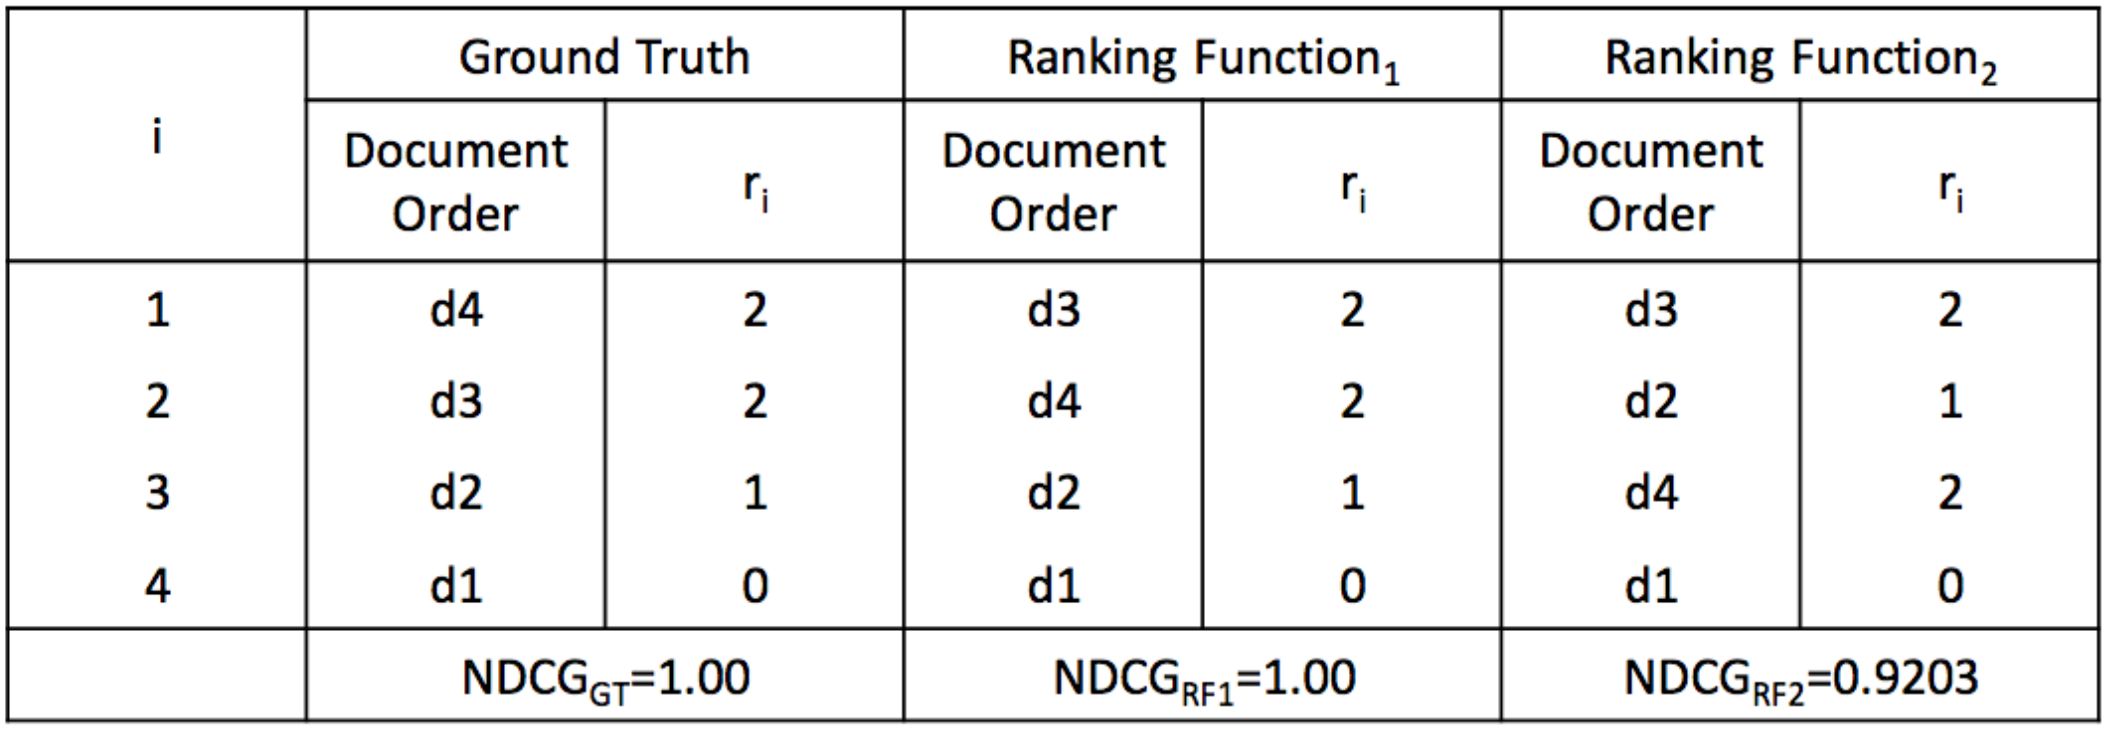
\includegraphics[width=.8\linewidth]{gfx/NDCGBeispiel}
		\vspace{-2em}
\end{minipage}
\hfill
\begin{minipage}{0.35\linewidth}
		\centering
		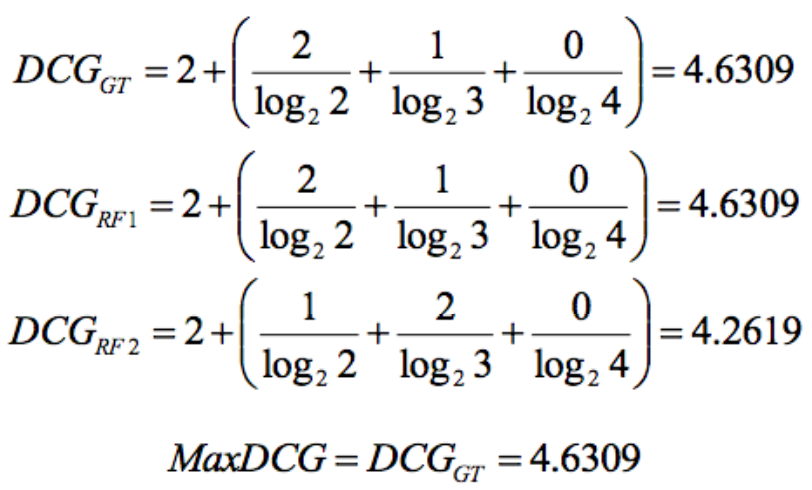
\includegraphics[width=.75\linewidth]{gfx/DCGBerechnung}
		\vspace{-3.5em}
\end{minipage}
\end{figure}

\subsection{Vorgehen}
\label{sec:Evaluation:Aufbau:Vorgehen}

\subsubsection{Testumgebung aufbauen}
\label{sec:Evaluation:Aufbau:Vorgehen:Aufbau}

Um eine Evaluation durchführen zu können, müssen wir eine passende Testumgebung aufbauen. Diese besteht aus einem Evaluations-System, einer Instanz der aktuellen Springermedizin-Applikation und einer Instanz des neu implementierten Lösungsansatzes. Auf dem Evaluations-System sollen fachliche Experten (Redakteure von Springermedizin) die Relevanz der Suchergebnisse der beiden Suchmaschinen vergleichen. Dazu sollen die jeweils ersten zehn Suchergebnisse nach Relevanz zum Suchterm bewertet werden. Der Ergebnisse werden in einer Datenbank gespeichert, um sie später auszuwerten. 

\paragraph{Aufbau des Evaluations-Systems}
Für die Analysen der Beurteiler implementieren wir selber ein kleines Evaluations-System als Web-Applikation. Das hat den Vorteil, dass wir selber definieren können, wie der Analyse-Prozess und wie die Datenstruktur der Analyse-Ergebnisse aussehen sollen. Das System umfasst eine Administrationsoberfläche zur Verwaltung der Analysedaten und eine Anwenderoberfläche zur Analyse der zugeteilten Suchterme. Der Beurteiler soll nur seine, ihm zugeteilten Suchterm-Analysen sehen. Um Analysen durchführen zu können, muss sich der Beurteiler darum an der Applikation anmelden. So können wir jedem Beurteiler ein eigenes Profil anlegen und ihm seine zu analysierenden Suchterme zuweisen. 

\paragraph{Verwendeter Technologiestack} 
Unser Evaluations-System werden wir wie die Springermedizin-Applikation (White Label Applikation) auf dem MVC-Framework \textit{Play}~\cite{Play} aufbauen und \textit{Scala}~\cite{Scala} als Programmiersprache verwenden. Um die Evaluationsdaten zu speichern verwenden wir eine PostgreSQL-Datenbank\footnote{PostgreSQL ist eine Objektrelationale Datenbank (ORDB)}~\cite{Postgresql}. Unsere beiden zu vergleichenden Springermedizin-Suchen bauen auf der Live-Applikation von Springermedizin auf und verwenden den Live-Content von Springermedizin zur Suche. Wir werden die beiden Suchen und das Evaluations-System darum in der Live-Umgebung der Springer Nature Cloud-Plattform Cloud Foundry\footnote{Cloud Foundry bietet Platform-as-a-Service  (PaaS) und ist eine Cloud die eine Computer-Plattform für Webanwendungen zur Verfügung stellt} laufen lassen. So haben wir ein realistisches Umfeld für die Evaluation. 

\paragraph{Analyse eines Suchterms}
Wir wollen zu jedem Suchterm eine Bewertung der aktuellen Springermedizin-Suche und eine, der Suche mit dem implementierten Reranking-Algorithmus. Wir bauen die Analysen darum so, dass der Benutzer beide Bewertungen nacheinander, in derselben Analyse ausführt. Zur Bewertung implementieren wir ein Maske, bestehend aus der zu beurteilende Suchvariante und einem Formular zur Bewertung der ersten zehn Suchresultate des Suchergebnisses. Die Bewertung besteht aus einer Skala von vier Relevanz-Werten, wobei \textit{nicht relevante} Ergebnisse bestraft werden sollen und darum einen negativen Relevanz-Wert erhalten:

\begin{table}[H]
\centering
\vspace{-.5em}
\caption[Relevanz-Werte für Bewertung der Suchresultate]{Relevanz-Werte für Bewertung der Suchresultate}
\label{tab:RelevanzWerteBewertungEvaluation}
\vspace{-.5em}
\footnotesize
\renewcommand*{\arraystretch}{1.2}
\begin{tabular}{llc}
\hline
\textbf{Relevanz}            & \textbf{Beschreibung}           & \textbf{Relevanz-Wert} \\ \hline
\textit{not relevant}        & Ergebnis hat \textbf{\textit{gar keine}} Relevanz & 0 \\
\textit{moderately relevant} & Ergebnis ist \textbf{\textit{eher irrelevant}}    & 1 \\
\textit{relevant}            & Ergebnis ist \textbf{\textit{eher relevant}}      & 2 \\
\textit{highly relevant}     & Ergebnis ist \textbf{\textit{sehr relevant}}      & 3 \\ \hline
\end{tabular}
\vspace{-2em}
\end{table}

Ist eine Bewertung gespeichert, wird die zweite Variante der Suche geladen. Eine Analyse ist dann abgeschlossen, wenn beide Suchvarianten bewertet sind. 

\pagebreak 

Der Ablauf einer Analyse sieht wie folgt aus:

\begin{figure}[H]
\centering
\vspace{-.5em}
\caption[Analyseprozess für Bewertung einer Suchvariante]{Analyseprozess für Bewertung einer Suchvariante}
\vspace{.5em}
\label{fig:AnalysemaskeEvaluation}
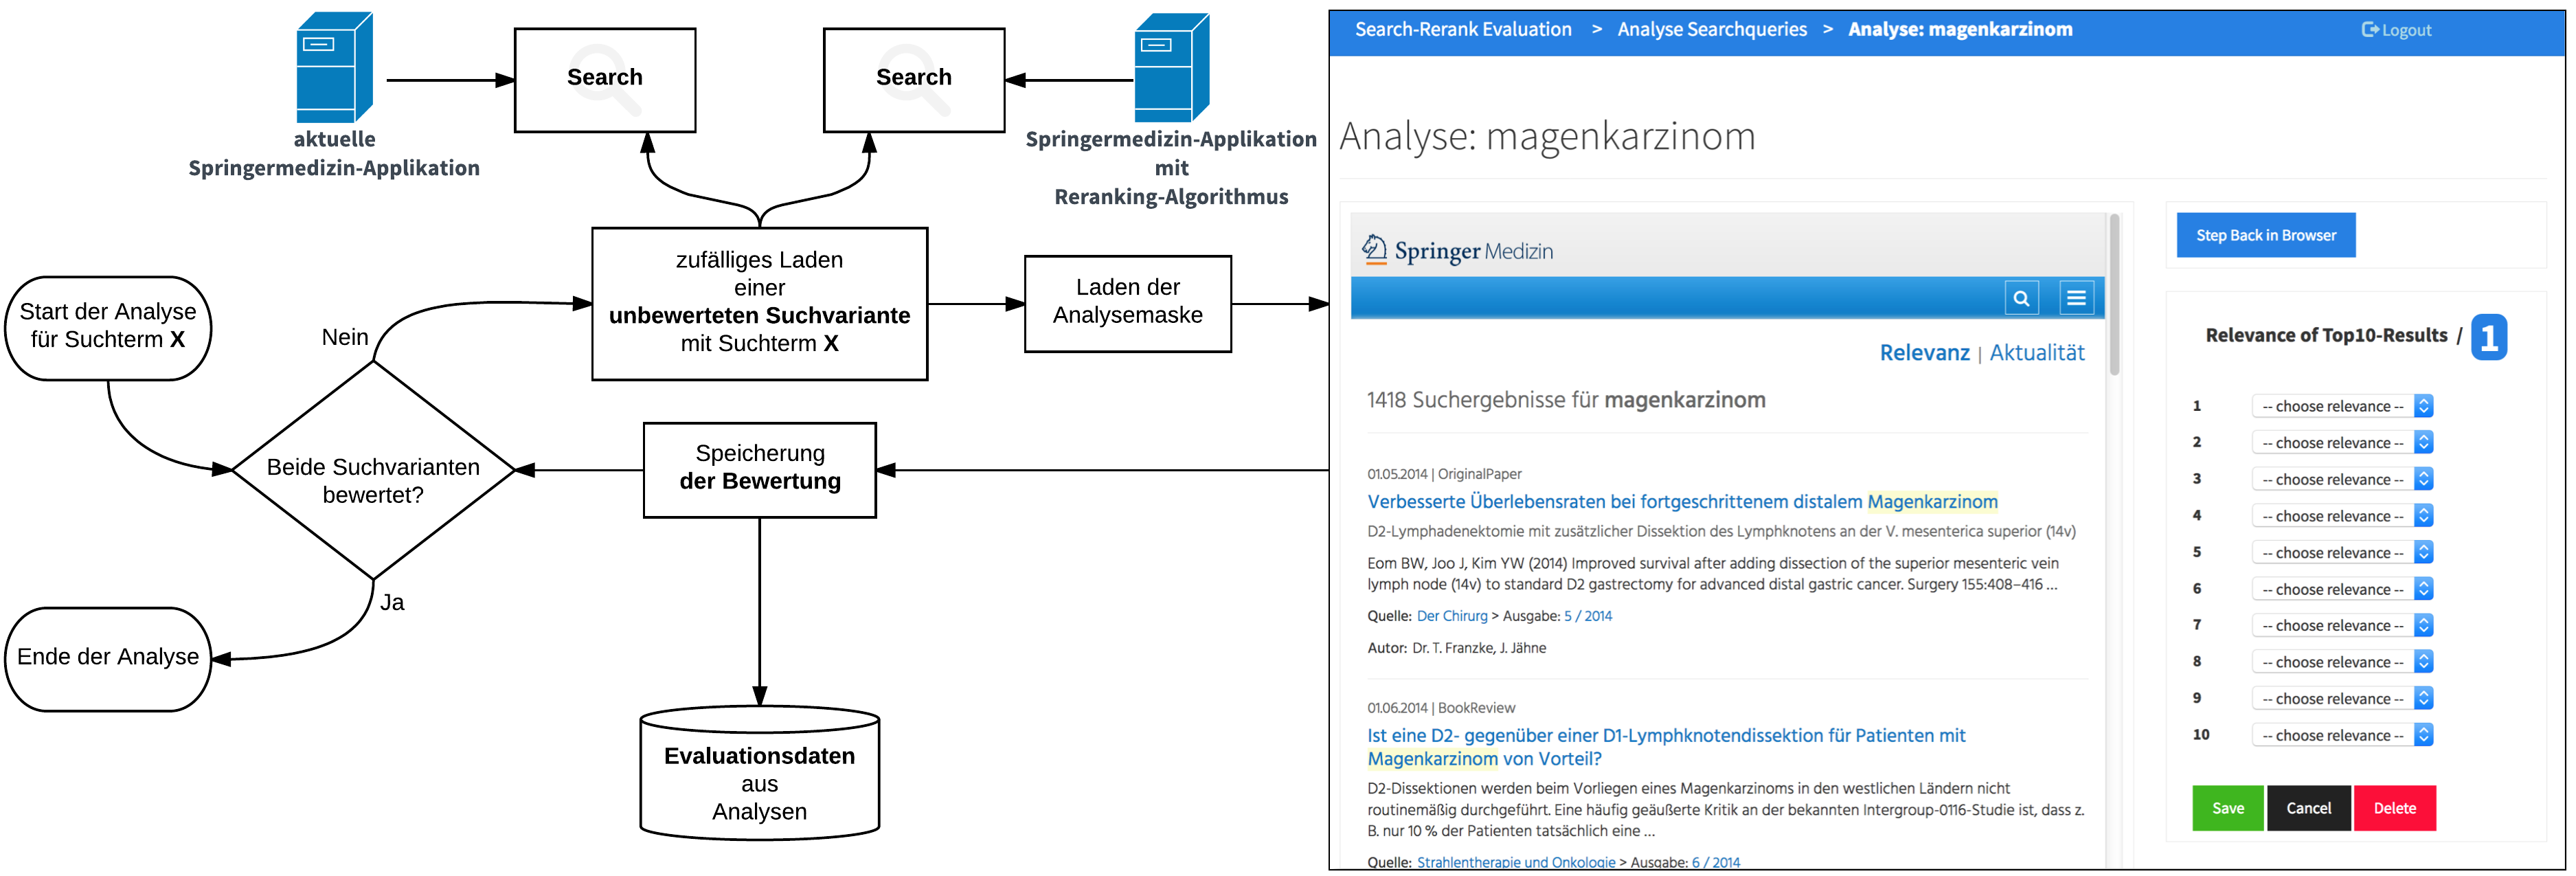
\includegraphics[width=\linewidth]{gfx/AnalysemaskeEvaluation}
\vspace{-1em}
\end{figure}

\subsubsection{Evaluations-Daten speichern}
\label{sec:Evaluation:Aufbau:Vorgehen:Speichern}

Zu jeder Analyse werden wir neben den Relevanz-Bewertungen und den Suchterm-Informationen auch wichtige Informationen zu den Click-Through-Daten und den Suchergebnissen speichern. Folgende Informationen liegen uns am Ende einer Analyse vor:

\begin{table}[H]
\centering
\vspace{-.5em}
\caption[Gespeicherte Evaluations-Daten zur Suchterm-Analyse]{Gespeicherte Evaluations-Daten zur Suchterm-Analyse}
\label{tab:EvaluationsDatenSpeicherung}
\vspace{-.5em}
\footnotesize
\renewcommand*{\arraystretch}{1.2}
\resizebox{\textwidth}{!}{%
\begin{tabular}{llll}
\hline
\textbf{Objekt}                                        & \textbf{Beide Suchvarianten}             & \textbf{Suche mit Reranking-Algorithmus} & \textbf{Beschreibung}                              \\ \hline
\multirow{4}{*}{\textit{\textbf{Analyse}}}             & \textit{Suchterm}                        & \textit{}                                & Analysierter Suchterm                              \\
                                                       & \textit{Beurteiler}                      & \textit{}                                & User-Informationen des Beurteilers                 \\
                                                       & \textit{Suchvariante}                    & \textit{}                                & Suche mit / ohne Reranking-Algorithmus             \\
                                                       & \textit{}                                & \textit{Wert des Zufallsfaktors}         & Einfluss-Wert Zufallsfaktor                        \\ \hline
\textit{\textbf{Bewertungen}}                          & \textit{Relevanz-Werte der Positionen}   & \textit{}                                & Relevanz-Bewertungen der ersten zehn Suchresultate \\ \hline
\multirow{2}{*}{\textit{\textbf{Click-Through-Daten}}} & \textit{}                                & \textit{User-Filter}                     & Alle Benutzer / eingeloggte Benutzer der Suche     \\
                                                       & \textit{}                                & \textit{Anzahl Klicks Gesamt}            & Anzahl gelesener Klicks aus Click-Through-Daten    \\ \hline
\textit{\textbf{Suchergebnis}}                         & \textit{Dokument-ID's der Suchresultate} & \textit{}                                & Dokument-ID's der ersten zehn Suchergebnisse       \\ \hline
\end{tabular}
}
\vspace{-2em}
\end{table}

\subsubsection{Evaluations-System auswerten}
\label{sec:Evaluation:Aufbau:Vorgehen:Auswerten}

Nach Abschluss der Evaluationsphase werden wir die Evaluations-Daten auswerten. Die Auswertung der Daten findet direkt im Evaluations-System statt. Dazu werden wir die Relevanz-Bewertungen aus der Datenbank lesen und wie oben beschrieben mit dem Cohens-Kappa-Koeffizienten und der nDCG-Metrik auswerten. Mithilfe der Evaluations-Daten können wir dann auch weitere Auswertungen zu den Click-Through-Daten und den Suchergebnissen der Suchterme machen.

\pagebreak

\subsection{Durchführung}
\label{sec:Evaluation:Aufbau:Durchfuehrung}

\subsubsection{Zu analysierende Suchterme}
\label{sec:Evaluation:Aufbau:Durchfuehrung:Aufgabenstellung}

Um die Evaluation praxisrelevant und mit genügend Click-Through-Daten ausführen zu können, wurden die Suchanfragen der letzten zwei Monate auf der Springermedizin-Suche analysiert und 80 oft gesuchte Suchterme ausgewählt (siehe Anhang \ref{sec:Anhang:VerwendeteSuchtermeEvaluation}). Springermedizin hat ein breites Spektrum an medizinischen Fachgebieten. Um fachlich gute Bewertungen zu kriegen, haben wir die Suchterme nach Fachrichtung unterteilt und jeweils zwei Beurteilern zugeteilt, die aus der Fachrichtung kommen:

\begin{table}[H]
\centering
\vspace{-.5em}
\caption[Fachrichtungen der Suchterme der Evaluation]{Fachrichtungen der Suchterme der Evaluation}
\label{tab:FachrichtungenSuchtermeEvaluation}
\vspace{-.5em}
\footnotesize
\renewcommand*{\arraystretch}{1.2}
\resizebox{\textwidth}{!}{%
\begin{tabular}{llc}
\hline
\textbf{Fachrichtung}            		& \textbf{Medizinisches Gebiet / Medizinischer Zweig}                  	& \multicolumn{1}{l}{\textbf{Anzahl zugeteilte Suchterme}} \\ \hline
\textit{Onkologie}               		& Tumorerkrankungen                                                    					& 10                                                       \\ \hline
\textit{Zahnmedizin}             		& Fachgebiet der Zahn-, Mund- und Kieferheilkunde                      		& 20                                                       \\ \hline
\textit{Gynäkologie}             		& Spezifischen Erkrankungen des weiblichen Körpers                    		& 10                                                       \\ \hline
\textit{AINS}                    			& Anästhesiologie, Intensivmedizin, Notfallmedizin und Schmerztherapie & 10                                                       \\ \hline
\textit{Neurologie, Psychiatrie} 	& Erkrankungen des Nervensystems und der Psyche                        	& 10                                                       \\ \hline
\textit{Innere Medizin}          		& Erkrankungen der inneren Organe                                      			& 10                                                        \\ \hline
\textit{Orthopädie}              		& Aufbau der Knochen und Muskeln des Menschen                          	& \multirow{3}{*}{10}                                      \\
\textit{Urologie}               			& Erkrankungen der Niere, Harnblase, Harnleiter und Harnröhre         	&                                                          \\
\textit{HNO}               				& Hals-Nasen-Ohren-Heilkunde                                           				&                                                          \\ \hline
\textbf{Gesamt:}                 		& \textbf{}                                                            							& \textbf{80}                                              \\ \hline
\end{tabular}
}
\vspace{-2em}
\end{table}

\subsubsection{Aufgabenstellung der Analyse}
\label{sec:Evaluation:Aufbau:Durchfuehrung:Aufgabenstellung}

Die Aufgabe der Analyse besteht darin, die jeweils ersten zehn Suchergebnisse nach Relevanz zum Suchterm zu bewerten. Insgesamt, soll jeder Beurteiler die ihm zugeteilten 20 Suchterme analysieren. Eine Analyse beinhaltet jeweils eine Bewertung des Suchterms, auf beiden Suchvarianten. In welcher Reihenfolge die Suchvarianten den Beurteilern während der Analyse präsentiert werden, ist rein \textit{zufällig} und \textit{variiert}. Es soll nicht ersichtlich sein, welche Variante jeweils bewertet wird. Dadurch können wir ausschließen, dass der Beurteiler durch die Bekanntgabe der Suchvariante subjektiv beeinflusst wird. 

\subsubsection{Verschiedene Varianten des neuen Lösungsansatzes evaluieren}
\label{sec:Evaluation:Aufbau:Durchfuehrung:EvaluationsdatenVarianteLoesungsansatzes}

Wie wir wissen, hat der Reranking-Algorithmus einige Faktoren, die variabel definiert werden können. Zu diesen Faktoren gehört der Einfluss des Zufallswertes in das Reranking ($\lambda$) und der \glqq Login-Status der User\grqq{} während der Suche, für die Selektion der Click-Through-Daten. Wir werden darum verschiedene Konstellationen testen, um die optimale Konstellation finden zu können. 

\paragraph{Definition der variablen Faktoren für den Reranking-Algorithmus}
Für den \textit{Einfluss des Zufallsfaktors} werden wir zwei Werte für $\lambda$ definieren. Diese sind 0.1 (zehn Prozent) und 0.05 (fünf Prozent). Für die \textit{Selektion der Click-Through-Daten} werden wir zwischen an der Applikation angemeldeten Benutzern und allen Benutzern (\textit{inkl. anonymen Benutzern}) unterscheiden. Aus den beiden Einflusswerten des Zufallsfaktors und der Unterscheidung zwischen angemeldeten und allen Benutzern, ergeben sich vier Konstellationen. Jeder Konstellation werden wir jeweils 25 Prozent der Suchterme zuteilen. Die Zuteilung der Suchterme werden wir mithilfe des Evaluations-Systems zufällig generieren lassen:

\begin{figure}[H]
\centering
\vspace{-.5em}
\caption[Aufteilung der Analysen für Evaluation]{Aufteilung der Analysen für Evaluation}
\vspace{.5em}
\label{fig:AufteilungAnalysenEvaluation}
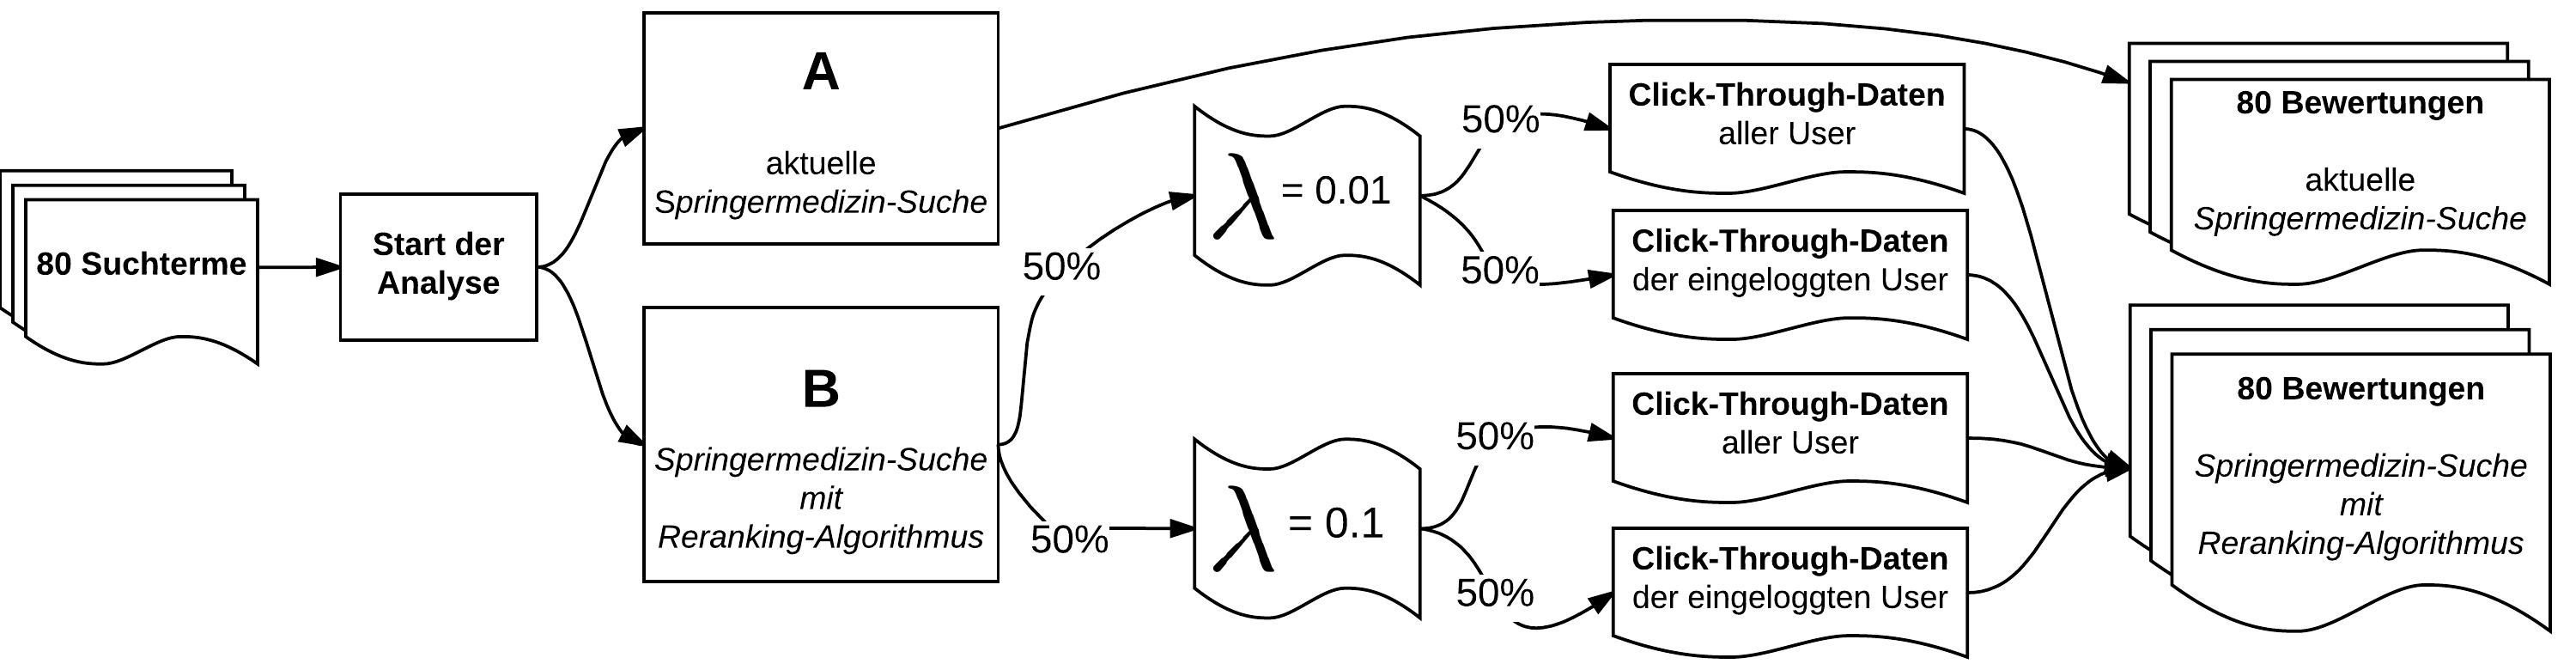
\includegraphics[width=0.9\linewidth]{gfx/EvaluationsvariantenRerankingSuche}
\vspace{-2em}
\end{figure}

\section{Auswertung der Suchergebnis-Qualität}
\label{sec:Evaluation:Auswertung}

Bei der Auswertung der Evaluationsdaten werden wir uns zuerst auf die Kappa-Werte fokussieren und analysieren, wie gut das Übereinstimmungsmaß $K_w$ der Beurteiler zu den Suchtermen ist. Danach folgt der Kern der Auswertung. Aus den Bewertungen, die das Mindestmaß für $K_w$ erfüllen, bestimmen wir das Qualitätsmaß der Suchvarianten mithilfe der nDCG-Metrik. Wir wollen herausfinden, welche Verbesserungen, mit welcher Konstellation des Reranking-Algorthmus möglich sind. Da der nDCG sich nur auf die Reihenfolge der Relevanz-Bewertungen konzentriert, wollen wir in einer weiteren Auswertung analysieren, welche durchschnittlichen Relevanz-Bewertungen die ersten zehn Suchresultate effektiv haben. So kriegen wir nicht nur ein Gefühl für die Ranking-Qualität der Suche sondern sehen auch gleich, wie gut die ausgespielten Ergebnisse effektiv sind. Zum Schluss werden wir die Einflüsse der Click-Through-Daten auf den nDCG analysieren und auswerten.

\subsection{Quantitative Auswertung}
\label{sec:Evaluation:Auswertung:QuantitativeAuswertung}

\subsubsection{Auswertung des Übereinstimmungsmaßes der Beurteiler mittels Kappa}
\label{sec:Evaluation:Auswertung:QuantitativeAuswertung:Kappa}

In dieser Analyse sehen wir, wie gut das Übereinstimmungsmaß $K_w$ der Beurteiler bei der Bewertung der Suchterme ist und wie viele der Suchterm-Bewertungen für die nDCG-Auswertung überhaupt in Frage kommen. 


\begin{figure}[H]
\centering 
\vspace{-1.5em}
\caption[Auswertungen des gewichteten Kappa $K_w$ der Suchterm-Bewertungen]{Auswertungen des gewichteten Kappa $K_w$ der Suchterm-Bewertungen}
\label{fig:Evaluation:Auswertung:Kappas}

\footnotesize
\pgfplotstableread[col sep=semicolon]{content/diagrams/eval/kappas.csv}\kappas
\pgfsetplotmarksize{.5pt}
  
\begin{tikzpicture}
\begin{axis}[
	width=14.5cm,
	height=4cm,
	scale only axis,
	xmajorgrids,
	xminorgrids,
    ylabel=\textbf{$K_w$}, 
	xlabel=\textbf{Suchterm-Analysen},
    xtick={0, 20, 40, 60, 80},
    ymin=0.3,
    xmin=0,
    xmax=80,
    y label style={yshift=-4mm},
    xlabel shift = 1in,
    ylabel shift = 1in,
   	legend style={at={(axis cs:1,0.325)},anchor=south west},
    legend style={font=\tiny},
    legend style={cells={align=left}}
]
\addplot table [
    y=Normal,
    x=Index
] {\kappas};
\addplot table [
    y=Rerank,
    x=Index
] {\kappas};
\addplot table [
    y=Grenzwert,
    x=Index,
    no marks
] {\kappas};
\legend{aktuelle Springermedizin-Suche, Suche mit Reranking-Algorithmus, {Grenzwert für Mindestmaß an $K_w$\\  (Übereinstimmungsgüte $\geq 0.60$)}}
\end{axis}
\end{tikzpicture}

\vspace{-2.5em}
\end{figure}

Die oben dargestellte Abb. \ref{fig:Evaluation:Auswertung:Kappas} zeigt ein Linien-Diagramm des Übereinstimmungsmaßes $K_w$ für die Relevanz-Bewertungen der Suchterme. Auf der x-Achse sehen wir die indexierte Reihenfolge der in der Evaluation verwendeten Suchterme, beginnend mit dem Index 0. Diese Suchterme können im Anhang unter \ref{sec:Anhang:VerwendeteSuchtermeEvaluation} nachgelesen werden. Die y-Achse zeigt die vertikale Messskala des gewichteten Kappa-Wertes $K_w$ und bewegt sich im Bereich zwischen 0 und 1. Die beiden Linien rot und blau stellen die $K_w$-Werte der Bewertungen der Suchterme der x-Achse in den zu vergleichenden Such-Implementierungen dar. Die blaue beschreibt hierbei die aktuelle Springemedizin-Suche und die rote stellt die Suche mit dem neu implementierten Reranking-Algorithmus dar. Die parallel zur x-Achse verlaufende, braune Linie stellt das Mindestmaß des $K_w$ dar. Aus diesem Diagramm können wir lesen, wie sich das Übereinstimmungsmaß eines Suchterms, zwischen den beiden Such-Implementierungen verändert. 

\paragraph{Beide Suchen zeigen ein sehr ähnliches Verhaltenmuster der Übereinstimmungsgüte} Wie wir sehen können, haben die Linien beider Such-Implementierungen mit Ausnahme vereinzelter Abweichungen, ein sehr ähnliches Verhaltensmuster. Die Abweichung der beiden Linien bewegen sich in den meisten Fällen, im Bereich von unter zehn Prozentpunkten. Die größten Abweichungen sind in den Suchtermen mit einem Index zwischen 50 und 60 sowie zwischen 70 und 80 zu erkennen. Das Mindestmaß an Übereinstimmung haben in beiden Such-Implementierungen 90 Prozent der Bewertungen erreicht. Bei der aktuellen Springermedizin-Suche waren die Resultate noch ein bisschen besser. Da haben nur sieben der 80 Bewertungen, das Mindestmaß nicht erreicht. Vereinzelt nähern sich die Kappa-Werte beider Suchen, stark dem maximalen Übereinstimmungswert von 1 an. 


\paragraph{Zum Vergleich der ungewichtete Kappa}
Wie bereits in der Datengrundlage im Kapitel \ref{sec:Evaluation:Aufbau:Datengrundlage} diskutiert, bewerten wir nicht den Cohens Kappa Koeffizienten $K$, sondern verwenden dessen gewichtete Variante $K_w$. Wir sind davon ausgegangen, dass die Wahrscheinlichkeit der genauen Übereinstimmung der Relevanz-Bewertung relativ klein ist, hingegen die der Bewertungen mit leichter Abweichung des Relevanz-Wertes, relativ groß sein könnte. Mithilfe dieser Analyse wollen wir herausfinden, ob wir mit unserer Vermutung richtig liegen.

\begin{minipage}{0.4\linewidth}
sadsdfsdf
\end{minipage}
\hfill
\begin{minipage}{0.55\linewidth}
\begin{figure}[H]
\centering 
\vspace{-1em}
\caption[Ungewichtete Kappa-Auswertung]{Ungewichtete Kappa-Auswertung}
\label{fig:Evaluation:Auswertung:KappasUnweighted}

\footnotesize
\pgfplotstableread[col sep=semicolon]{content/diagrams/eval/kappasUnweighted.csv}\kappas
\pgfsetplotmarksize{.5pt}
  
\begin{tikzpicture}
\begin{axis}[
	width=7cm,
	height=4cm,
	scale only axis,
	xmajorgrids,
	xminorgrids,
    ylabel=\textbf{$K_w$}, 
	xlabel=\textbf{Suchterm-Analysen},
    xtick={0, 20, 40, 60, 80},
    xmin=0,
    xmax=80,
    xlabel shift = 1in,
    ylabel shift = 1in,
    legend style={font=\tiny},
    legend style={at={(axis cs:20,-0.75)},anchor=south west}
]
\addplot table [
    y=Normal,
    x=Index
] {\kappas};
\addplot table [
    y=Rerank,
    x=Index
] {\kappas};
\addplot table [
    y=Grenzwert,
    x=Index,
    no marks
] {\kappas};
\legend{aktuelle Springermedizin-Suche, Suche mit Reranking-Algorithmus, Grenzwert ($0.60$)}
\end{axis}
\end{tikzpicture}

\vspace{-2.5em}
\end{figure}
\end{minipage}


\subsubsection{Bestimmung des Qualitätsmaßes der Suchvarianten durch nDCG-Auswertungen}
\label{sec:Evaluation:Auswertung:QuantitativeAuswertung:nDCG}

In der folgenden Analyse werden wir nun sehen, welche Suchvariante des Reranking-Algorithmus die beste Konstellation darstellt und welche Verbesserung der Ranking-Qualität der Suche, das Reranking der Suchresultate bewirkt. Wir vergleichen dazu den durchschnittlichen nDCG-Wert der jeweiligen Suchvariante des Reranking-Algorithmus, mit dem durchschnittlichen nDCG-Wert der aktuellen Springermedizin-Suche. Bei der Evaluation haben wir immer die ersten zehn Suchresultate verglichen. Wir berechnen darum den $nDCG_{10}$ der Suchterme für die Auswertung.


\begin{figure}[H]
\centering 
\vspace{-1.5em}
\caption[nDCG-Auswertung]{nDCG-Auswertung aller Suchvarianten}
\label{fig:Evaluation:Auswertung:NDCGVarianten}

\footnotesize
\pgfplotstableread[col sep=semicolon]{content/diagrams/eval/nDCG.csv}\ndcg
\pgfsetplotmarksize{.5pt}

\begin{tikzpicture}
\begin{axis}[
	ybar,
    ymin=0,
    ymax=1.1,
	xtick=data,
	xticklabel style={align=center},
	xticklabels={{$\lambda$ für $X_u: 0.05$ \\ CTR aller \textit{angemeldeten User}}, {$\lambda$ für $X_u: 0.05$ \\ CTR \textit{aller User}}, {$\lambda$ für $X_u: 0.1$ \\ CTR aller \textit{angemeldeten User}}, {$\lambda$ für $X_u: 0.1$ \\ CTR \textit{aller User}}},
	width=11cm,
	height=4cm,
	scale only axis,
	ymajorgrids,
	yminorgrids,
	y label style={yshift=-4mm},
	x label style={yshift=-5mm},
    ylabel=\textbf{$nDCG_{10}$}, 
	xlabel=\textbf{Suchvarianten des Reranking-Algorithmus},
    legend style={font=\tiny},
   	legend pos=outer north east,
   	 legend style={cells={align=left}}
]
\addplot[nodes near coords, 
	every node near coord/.append style={xshift=-5pt,yshift=-1pt}, draw = blue,
       fill = blue!30!white] plot table [
    y=AVG_S,
    x=Index
] {\ndcg};
\label{pgfplots:plot1}
%\addlegendentry{$nDCG_{10}$ der aktuellen \\ Springermedizin-Suche}
\addplot[nodes near coords, 
	every node near coord/.append style={xshift=5pt,yshift=-1pt}, draw = red,
       fill=red!30!white] plot table [
    y=AVG_R,
    x=Index
] {\ndcg};
\label{pgfplots:plot2}
%\addlegendentry{$nDCG_{10}$ der Variante der Suche\\ mit dem Reranking-Algorithmus}
\end{axis}
\begin{axis}[
    ymin=0,
    ymax=1.1,
	xtick=\empty,
	ytick=\empty,
	width=11cm,
	height=4cm,
	scale only axis,
	ymajorgrids,
	yminorgrids,
    legend style={font=\tiny},
   	legend pos=outer north east
]
\addplot[draw=blue] plot table [
    y=AVG_S_Min,
    x=Index
] {\ndcg};
\label{pgfplots:plot3}
\addplot[draw=red] plot table [
    y=AVG_R_Min,
    x=Index
] {\ndcg};
\label{pgfplots:plot4}
\addplot[draw=blue] plot table [
    y=AVG_S_Max,
    x=Index
] {\ndcg};
\addplot[draw=red] plot table [
    y=AVG_R_Max,
    x=Index
] {\ndcg};
\end{axis}

%Legende
\matrix[
    matrix of nodes,
    anchor=north west,
    draw,% Rahmen um Legende
    inner sep=0.2em,
    column 1/.style={nodes={anchor=center}},
    column 2/.style={nodes={anchor=west},font=\tiny,cells={align=left}},
    draw
  ]    
at([xshift=0.25cm]current axis.north east){
    \ref{pgfplots:plot1}& $nDCG_{10}$ der aktuellen \\
    & Springermedizin-Suche\\
    & \ \\
    \ref{pgfplots:plot2}& $nDCG_{10}$ der Suchvariante \\ 
    & mit dem Reranking-Algorithmus\\
    & \ \\
    \ref{pgfplots:plot3}& Minimal- und Maximalwert des\\ 
    & $nDCG_{10}$ der aktuellen \\
    & Springermedizin-Suche\\
    & \ \\
    \ref{pgfplots:plot4}& Minimal- und Maximalwert des\\ 
    & $nDCG_{10}$ der Suchvariante \\ 
    & mit dem Reranking-Algorithmus\\};
\end{tikzpicture}


\vspace{-2.5em}
\end{figure}

Die oben dargestellte Abb. \ref{fig:Evaluation:Auswertung:NDCGVarianten} zeigt eine Mischform von einem Säulen- und Liniendiagramm. Die Säulen bezeichnen hierbei jeweils die verwendete Such-Implementierung. Die blauen Säulen beschreiben den durchschnittlichen $nDCG_10$ der aktuellen Springermedizin-Suche. Die roten stellen jeweils den durchschnittlichen $nDCG_10$  einer Suchvariante der Suche mit dem Reranking-Algorithmus dar. Die Werte der x-Achse beschreiben hierbei, welche dieser Suchvarianten, jeweils mit der aktuellen Springermedizin-Suche verglichen wird. Der Faktor $\lambda$ für $X_u$ zeigt jeweils den Einfluss des Zufallswertes in den Reranking-Algorithmus und CTR beschreibt die Filterung der Click-Through-Daten anhand des Login-Status, bei der Berechnung der CTR. Die y-Achse beschreibt die Werteskala der nDCG-Auswertung. Diese bewegt sich zwischen 0 und 1. Die Linien stellen jeweils die Minimal- und Maximalwerte der gleichfarbigen Säulen dar.

\paragraph{Der Reranking-Algorithmus weist leichte Verbesserungen gegenüber der aktuellen Suche auf}
Wie wir sehen, liegen alle nDCG-Werte nahe beieinander. Die größten Verbesserungen weist der kleinere Einflussfaktor $\lambda$ für $X_u$~(0.05) des Zufallswertes, in Verbindung mit den Click-Through-Daten der angemeldeten User auf. Die einzige Verschlechterung mittels Reranking-Algorithmus, tritt bei der Verwendung des höheren Einflussfaktors $\lambda$ für $X_u$ und der Berechnung der CTR aus den Click-Through-Daten aller User auf. Die Minimal- und Maximalwerte der beiden Suchen verhalten sich sehr ähnlich zu einander. Nur die letzte Konstellation, welche bereits beim durchschnittlichen nDCG-Wert Verschlechterungen zeigt, weist eine leichte Abweichung der Minimalwerte auf. Hingegen nähern sich alle Maximalwerte des nDCG, stark dem Maximalwert von 1 an. Anhand der Differenz der Minimalwerte der Suchvarianten können wir feststellen, dass der größere Einfluss-Faktor des Zufallswertes $\lambda$ für $X_u$, bessere Minimalwerte erzeugt.

\paragraph{Effektive Relevanz-Bewertungen aller Suchvarianten vergleichen}
In der unten folgenden Abb. \ref{fig:Evaluation:Auswertung:RelevanzVarianten} vergleichen wir, wie relevant die Dokumente der Suchergebnisse zum Suchterm effektiv waren. Dazu berechnen wir den durchschnittlichen Relevanz-Wert der Positionen zu jeder Suchvariante.


\begin{figure}[H]
\centering 
\vspace{-1em}
\caption[Durchschnittliche Relevanz-Werte der Suchvarianten für die ersten zehn Suchpositionen]{Durchschnittliche Relevanz-Werte der Suchvarianten für die ersten zehn Suchpositionen}
\label{fig:Evaluation:Auswertung:RelevanzVarianten}

\footnotesize
\pgfplotstableread[col sep=semicolon]{content/diagrams/eval/relevanceVarianten.csv}\rel
  
\begin{tikzpicture}
\begin{axis}[
	width=11cm,
	height=4cm,
	scale only axis,
	xmajorgrids,
	xminorgrids,
    ylabel=\textbf{Relevanz-Wert}, 
	xlabel=\textbf{Position},
    xtick=data,
    xlabel shift = 1in,
    ylabel shift = 1in,
    xmin=1,
	xmax=10,
    y label style={yshift=-4mm},
   	legend pos=outer north east,
    legend style={font=\tiny},
    legend style={cells={align=left}}
]
\addplot table [
    y=N,
    x=Position
] {\rel};
\addplot table [
    y=R1,
    x=Position
] {\rel};
\addplot table [
    y=R2,
    x=Position
] {\rel};
\addplot table [
    y=R3,
    x=Position
] {\rel};
\addplot table [
    y=R4,
    x=Position
] {\rel};
\legend{aktuelle Springermedizin-Suche, {Reranking-Algorithmus mit:\\$\lambda$ für $X_u: 0.05$ \\ CTR aller \textit{angemeldeten User}}, {Reranking-Algorithmus mit:\\$\lambda$ für $X_u: 0.05$ \\ CTR \textit{aller User}}, {Reranking-Algorithmus mit:\\$\lambda$ für $X_u: 0.1$ \\ CTR aller \textit{angemeldeten User}}, {Reranking-Algorithmus mit:\\$\lambda$ für $X_u: 0.1$ \\ CTR \textit{aller User}}}
\end{axis}
\end{tikzpicture}

\vspace{-2em}
\end{figure}

Die oben sichtbare Darstellung eines Liniendiagramms, stellt die ersten zehn Positionswerte aller Suchvarianten miteinander ins Verhältnis. Die x-Achse beschreibt hierbei die dargestellte Position im Suchergebnis. Die y-Achse zeigt den Relevanz-Wert, mit welchem die Suchergebnisse auf dieser Position durchschnittlich bewertet werden. Der Relevanz-Wert kann einen Wert von minimal 0 bis und maximal 3 annehmen. Die Relevanz-Werte der Suchvarianten bewegen sich in einem Bereich zwischen 1 und 2.5 . Die farbigen Linien beschreiben jeweils die Relevanz-Bewertungen für entweder die Springermedizin-Suche oder eine der verschiedenen Suchvarianten der Suche mit dem Reranking-Algorithmus. 

\paragraph{Suchvarianten mit CTR der angemeldeten User weisen die besseren Relevanz-Werte auf}
Wie bereits in der Auswertung des nDCG in Abb. \ref{fig:Evaluation:Auswertung:NDCGVarianten}, weist die Suchvariante des Reranking-Algorithmus mit dem kleineren Einfluss-Faktors $\lambda$ für $X_u$ und der CTR der angemeldeten User, die höchsten Relevanz-Bewertungen auf. Die aktuelle Springermedizin-Suche hat eine fast linear abfallende Form der Relevanz-Werte. Sehr ähnlich verhält sich die vierte Suchvariante des Reranking-Algorithmus, mit dem größeren Einfluss-Faktor $\lambda$ für $X_u$ und der CTR aller User. Die schlechteste Konstellation der Suchvarianten des Reranking-Algorithmus, stellt die braune Linie mit dem kleineren Einfluss $\lambda$ für $X_u$ und der CTR aller User dar. Diese fällt ab Position fünf stark ab.

\subsubsection{Auswertung des Einflusses der Click-Through-Daten auf den nDCG}
\label{sec:Evaluation:Auswertung:QuantitativeAuswertung:EinflussNDCG}

Mit den unten folgenden Analysen untersuchen wir den Einfluss der Anzahl der Click-Through-Daten auf das Ergebnis der nDCG-Auswertung. Für die erste Analyse vergleichen wir die Anzahl der Klicks, die Gesamthaft zum Suchterm zur Verfügung stehen, mit den resultierenden nDCG-Werten. Die blaue Linie mit dem durchschnittlichen nDCG-Wert aller Suchvarianten des Reranking-Algorithmus, dient hier als Richtwert.

\begin{minipage}{0.40\linewidth}
Auf der rechts dargestellten Abb. beschreibt die x-Achse die Anzahl der gefundenen Klicks, für die Berechnung des CTR mittels Reranking-Algorithmus. Die y-Achse beschreibt den nDCG-Wert, der aus dem Reranking-Algorithmus resultierenden Suchergebnisliste. Das Verhalten der nDCG-Werte abhängig der Anzahl Klicks, zeigt ein sehr sprunghaftes Verhalten, wobei sich die nDCG-Werte in den meisten Fällen im Bereich zwischen 0.7 und 1 bewegen. Ein sehr schwacher nDCG-Wert ist die Ausnahme und nur bei der Klickanzahl 65 zu sehen.
\end{minipage}
\hfill
\begin{minipage}{0.55\linewidth}
\begin{figure}[H]
\centering 
\vspace{-1.5em}
\caption[Click-Through-Daten: Einfluss der Anzahl Klicks gesamt auf $nDCG$]{Click-Through-Daten: Einfluss der Anzahl Klicks gesamt auf $nDCG$}
\label{fig:Evaluation:Auswertung:ClicksNDCG}

\footnotesize
\pgfplotstableread[col sep=semicolon]{content/diagrams/eval/clicksNDCG.csv}\clicks
\pgfsetplotmarksize{.5pt}
  
\begin{tikzpicture}
\begin{axis}[
	width=8cm,
	height=3.5cm,
	scale only axis,
	xmajorgrids,
	xminorgrids,
    ylabel=\textbf{$nDCG$}, 
	xlabel=\textbf{Anzahl Klicks},
    xtick={0,20,40,60,80,100},
   	xmin=0,
	xmax=100,
    xlabel shift = 1in,
    ylabel shift = 1in,
    y label style={yshift=-4mm},
    legend style={font=\tiny},
    legend style={at={(axis cs:100,0)},anchor=south east}
]
\addplot table [
    y=AVG,
    x=Klicks
] {\clicks};
\addplot table [
    y=NDCG,
    x=Klicks
] {\clicks};
\legend{Durchschnittlicher $nDCG$, $nDCG$ abhängig der Anzahl Klicks gesamt}
\end{axis}
\end{tikzpicture}

\vspace{-2.5em}
\end{figure}
\end{minipage}


\begin{minipage}{0.40\linewidth}
Bei der rechts folgenden Abb. werden wir wie in der oberen Abb. \ref{fig:Evaluation:Auswertung:ClicksNDCG}, die Einflüsse der Click-Through-Daten messen. Nur dieses Mal vergleichen wir die Diversität der angeklickten Positionen, mit deren Einfluss auf den nDCG. Wie wir an der roten Linie erkennen, haben die Click-Through-Daten mit weniger als 20 unterschiedlichen Positionen, tendenziell die besten nDCG-Werte. Die Positionszahlen dahinter verhalten sich sehr sprunghaft und weisen viele schwache nDCG-Werte auf.
\end{minipage}
\hfill
\begin{minipage}{0.55\linewidth}
\begin{figure}[H]
\centering 
\vspace{-1em}
\caption[Click-Through-Daten: Einfluss der Anzahl unterschiedlicher Positionen auf nDCG]{Click-Through-Daten: Einfluss der Anzahl unterschiedlicher Positionen auf nDCG}
\label{fig:Evaluation:Auswertung:RanksNDCG}

\footnotesize
\pgfplotstableread[col sep=semicolon]{content/diagrams/eval/ranksNDCG.csv}\ranks
\pgfsetplotmarksize{.5pt}
  
\begin{tikzpicture}
\begin{axis}[
	width=8cm,
	height=3.5cm,
	scale only axis,
	xmajorgrids,
	xminorgrids,
    ylabel=\textbf{$nDCG$}, 
	xlabel=\textbf{Anzahl unterschiedlicher Positionen},
    xtick={0,20,40,60,80},
   	xmin=0,
	xmax=80,
    xlabel shift = 1in,
    ylabel shift = 1in,
    y label style={yshift=-4mm},
    legend style={font=\tiny},
    legend style={at={(axis cs:80,0)},anchor=south east}
]
\addplot table [
    y=AVG,
    x=Positionen
] {\ranks};
\addplot table [
    y=NDCG,
    x=Positionen
] {\ranks};
\legend{Durchschnittlicher $nDCG$, $nDCG$ abhängig der Anzahl unterschiedlicher Positionen}
\end{axis}
\end{tikzpicture}

\vspace{-2em}
\end{figure}
\end{minipage}


\subsection{Diskussion}
\label{sec:Evaluation:Auswertung:Diskussion}

\subsubsection{Auswertung des Übereinstimmungsmaßes der Beurteiler mittels Kappa}
\label{sec:Evaluation:Auswertung:Diskussion:Kappa}

\subsubsection{Bestimmung des Qualitätsmaßes der Suchvarianten durch nDCG-Auswertungen}
\label{sec:Evaluation:Auswertung:Diskussion:nDCG}


\subsubsection{Auswertung des Einflusses der Click-Through-Daten auf den nDCG}
\label{sec:Evaluation:Auswertung:Diskussion:EinflussNDCG}

\section{Zusammenfassung}
\label{sec:Evaluation:Zusammenfassung}

%--------------------

%\paragraph{Manche Suchbegriffe sind aus meiner Sicht zu allgemein ( „operative Therapie“) oder veraltet („Prostata-Adenom“ statt benigne „Prostatahyperplasie“)%
